\ofsubsection{Tumba de Raithwall}
%
\ofquote{"Embora seja chamado de o Rei Dinástico, ao estabelecer a aliança, mostrou compaixão pelo seu povo e desprezo pela guerra. Uma filosofia foi passada a seus sucessores. Aquele que traria paz e prosperidade pelos séculos vindouros."}{Ashe}\\\\
%
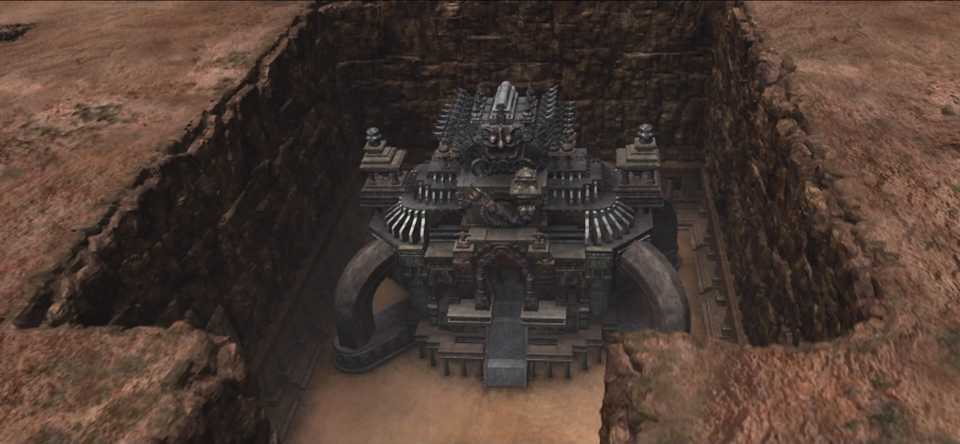
\includegraphics[width=\columnwidth]{./art/tombofraithwall/tomb1.jpg}
%
\ofpar
%
\accf{Tumba de Raithwall} é uma aventura preparada independente, que pode ser jogada tanto avulsa quanto parte de uma campanha maior. 
Nela, o grupo explora uma antiga tumba em busca de um poderoso artefato lendário.
A Tumba de Raithwall é projetada para um grupo de nível 3, mas a depender dos fatores como tamanho e experiencia do grupo, talvez seja necessário adaptar alguns dos inimigos e recompensas.
Caso os jogadores criem personagens de nível 3, eles podem usar as regras padrão para escolha de equipamento e cada um recebe 1.500G adicionais.
Além disso, a história de cada um deles deve explicar o porque deles se juntarem nesta perigosa caçada ao tesouro.
%
\ofpar
%
\ofquote{"Não há garantia que sairemos com vida? Bestas malígnas. Armadilhas malditas. Algo parecido?"\\}{Balthier}\\\\
%
Após uma marcha através do vasto mar de areia de Nam-Yensa, o grupo se encontra perante um alto penhasco e percebem uma passagem estreita adentrando.
Próxima à entrada, eles encontram um marcador viajante \accf{Dyce} em seu acampamento montado.
Dyce é um homem atlético, alto, careca, barbudo e usa vestes negras, ele também tem uma Chocobo ao seu lado, na qual viaja.
Ele informa ao grupo que o caminho através do penhasco leva a Tumba de Raithwall e lhes conta a história dele: a tumba é o local de repouso do \accf{Rei Raithwall}, também chamado de Rei Dinástico.
As lendas dizem que em tempos antigos, Raithwall foi um rei generoso que uniu muitos reinos em guerra sob seu estandarte, trazendo paz e prosperidade às terras.
Acredita-se que a chave para seu poder era um artefato mágico, chamado de \accf{Fragmento da Aurora}.
Segundo a lenda, como seu último ato, ele selou a tumba consigo e com o fragmento da aurora a fim de prevenir que seu poder caísse em mãos erradas.
Muitos aventureiros tentaram reivindicar o fragmento da aurora, mas somente encontraram seu fim perante os muitos perigos e armadilhas da tumba.
Com mais investigação, o grupo pode descobrir que Dyce não está aqui por coincidência, na verdade ele está esperando lucrar com os muitos aventureiros passando por ali.
Assim, ele também oferece vender suas mercadorias ao grupo a um preço 50\% maior do que o normal (ele chama isso de "prêmio de risco").
Ele tem os seguintes itens e acessórios em seu inventário: poção, éter, poção maior, super éter, pena de fênix, cortina de luz, cortina lunar, braçadeira rúnica, escudo mithril, óculos prata, capa branca e pendente estelar.
%
\vfill
%
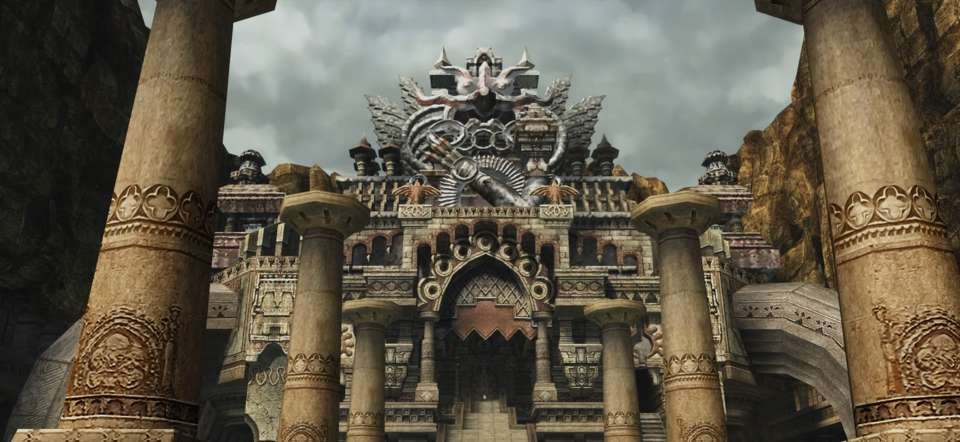
\includegraphics[width=\columnwidth]{./art/tombofraithwall/tomb2.jpg}
%
\vfill
%
Após o grupo por os pés na estreita abertura no penhasco, eles se encontram no conhecido \accf{Vale da Morte} com a enorme tumba em frente a eles.
Um conjunto de altos pilares de pedra em ambos os lados marcam o caminho até um longo lance de escadas que levam à Tumba de Raithwall.
À medida em que o grupo cobre metade do caminho até as escadas, de repente são atingidos por um guincho ensurdecedor vindo de uma criatura parecida com um pássaro, desce sobre eles.
\accf{Garuda} como um dos vários guardiões da tumba, protege a entrada durante a batalha a seguir.
Somente depois de derrotar a besta, o grupo pode entrar na tumba através do lance central de escadas.
%
\vfill
%
\ofmonster{Garuda}{3}{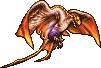
\includegraphics[width=0.3\columnwidth]{./art/tombofraithwall/garuda.jpg}}
{
	PV: & \hfill 60 & PM: & \hfill 80\\
	FOR: & \hfill 3 & DEF: & \hfill 2 \\
	MAG: & \hfill 4 & RES: & \hfill 3 \\
	AGI: & \hfill 2 & Tamanho: & \hfill G\\
}
{\accf{Bico}: 2d Dano\hfill \accf{Deixa:} 800G, Pena de Fênix\\ \accf{Resistente:}\wind \hfill \accf{Imune:}\poison\sleep\immobile \hfill \accf{Fraco:\lightning}}
{
	\mspell{Aero}{8}{0r}{Único}{4u}{Cause 2d de dano de Vento ao alvo.}{\wind}
	\mspell{Explosão Aérea}{10}{1r}{10u (linha)}{Você}{Inimigos na área sofrem 4d de dano de Vento.}{\wind}
	\mtech{Voar}{4}{0r}{Único}{Você}{Suba até uma altura de 3u. enquanto no ar, mova-se normalmente. Após 4 rodadas, desça ao lado de um inimigo dentro de 8u e o ataque.}{}
	\mpassive{Tapa de asa}{Sempre que atacar um inimigo ao alcance, você também pode atacar outro inimigo dentro de 2u.}
}
%
\clearpage
%
\ofquote{"Lutar ou fugir, melhor decidir logo!"\\}{Vaan}
%
\vfill
%
\colorlet{tombfloor}{yellow!10!white}
\colorlet{tombwall}{white!50!brown}
\colorlet{tombobstacle}{brown}
\colorlet{tombobject}{white!80!black}
\resizebox{\columnwidth}{!}{
	\centering
	\begin{tikzpicture}[]
	\tikzstyle{stairs}=[fill=tombfloor, ultra thick, draw, trapezium, trapezium angle=85, align=center, pattern=horizontal lines]
	\tikzstyle{pillar}=[ultra thick, draw, circle, align=center, fill=tombobstacle, minimum height=0.05\textwidth]
	\tikzstyle{room}=[fill=tombfloor, ultra thick, draw, rectangle, align=center]
	\tikzstyle{door}=[fill=tombobstacle, ultra thick, draw, rectangle, align=center]
	
	\node[ultra thick, fill=tombwall, draw, rectangle, minimum height=\textheight, minimum width=\textwidth](tarea)at (0,0) {};
	
	\node[fill=yellow!30!white, ultra thick, draw, rectangle, align=center, minimum height=0.2\textheight, minimum width=\textwidth](a1)at (0\textwidth, -0.4\textheight) {};
	
	\node[room, minimum height=0.175\textheight, minimum width=0.7\textwidth](a1)at (0\textwidth, 0.37\textheight) {};
	\node[room, minimum height=0.175\textheight, minimum width=0.8\textwidth](a1)at (0\textwidth, -0.1375\textheight) {};
	\node[room, minimum height=0.05\textheight, minimum width=0.8\textwidth](a1)at (0\textwidth, -0.025\textheight) {};
	\node[room, minimum height=0.28\textheight, minimum width=0.2\textwidth](a1)at (0\textwidth, 0.14\textheight) {};
	
	
	\node[fill=tombfloor, ultra thick, draw, trapezium, trapezium angle=85, align=center, rotate=180, minimum height=0.075\textheight](a1)at (0\textwidth, -0.2625\textheight) {};
	\node[stairs, rotate=180, minimum height=0.075\textheight](a1)at (0\textwidth, -0.2625\textheight) {};
	\node[stairs, minimum height=0.05\textheight](a1)at (-0.3\textwidth, -0.075\textheight) {};
	\node[stairs, minimum height=0.05\textheight](a1)at (0.3\textwidth, -0.075\textheight) {};	
	\node[stairs, pattern=vertical lines, rotate=90, minimum height=0.05\textheight](a1)at (-0.3125\textwidth, 0.37\textheight) {};
	\node[stairs, pattern=vertical lines, rotate=270, minimum height=0.05\textheight](a1)at (0.3125\textwidth, 0.37\textheight) {};
	
	\node[door, minimum height=0.01\textheight, minimum width=0.2\textwidth](a1)at (0\textwidth, 0.28\textheight) {};
	\node[door, minimum height=0.01\textheight, minimum width=0.15\textwidth](a1)at (0\textwidth, 0.455\textheight) {};
	
	\node[pillar, minimum height=0.02\textheight](a1)at (0.2\textwidth, -0.475\textheight) {};
	\node[pillar, minimum height=0.02\textheight](a1)at (0.2\textwidth, -0.4\textheight) {};
	\node[pillar, minimum height=0.02\textheight](a1)at (0.2\textwidth, -0.325\textheight) {};
	\node[pillar, minimum height=0.02\textheight](a1)at (-0.2\textwidth, -0.475\textheight) {};
	\node[pillar, minimum height=0.02\textheight](a1)at (-0.2\textwidth, -0.4\textheight) {};
	\node[pillar, minimum height=0.02\textheight](a1)at (-0.2\textwidth, -0.325\textheight) {};
	
	\node[fill=tombobject, ultra thick, draw, rectangle, align=center, minimum height=0.02\textheight, minimum width=0.2\textwidth](demonwall)at (0\textwidth, -0.05\textheight) {};
	
	\draw[tombfloor, -, ultra thick](-0.1\textwidth, 0\textheight) -- (0.1\textwidth, 0\textheight);
	\draw[tombfloor, -, ultra thick](0.335\textwidth, -0.05\textheight) -- (0.265\textwidth, -0.05\textheight);
	\draw[tombfloor, -, ultra thick](-0.335\textwidth, -0.05\textheight) -- (-0.265\textwidth, -0.05\textheight);	
	\draw[tombfloor, -, ultra thick](0.355\textwidth, -0.1\textheight) -- (0.245\textwidth, -0.1\textheight);
	\draw[tombfloor, -, ultra thick](-0.355\textwidth, -0.1\textheight) -- (-0.245\textwidth, -0.1\textheight);
	
	
	\node[align=center](a2)at (0.4\textwidth, -0.4\textheight) {\bf\LARGE Vale da \\\\ \bf\LARGE Morte};	
	\node[align=center](a2)at (0.25\textwidth, 0.075\textheight) {\bf\LARGE Salão do \\\\ \bf\LARGE Destruidor};
	
	\node[align=center](a2)at (0.425\textwidth, 0.37\textheight) {\bf\Large Passagem  \\ \bf\Large da Queda \\ \bf\Large norte};
	\node[align=center](a2)at (-0.425\textwidth, 0.37\textheight) {\bf\Large Passagem\\ \bf\Large da Queda \\ \bf\Large sul};
	\node[align=center](a2)at (0\textwidth, 0.33\textheight) {\bf\Large Câmara Real};
	\node[align=center](a2)at (0\textwidth, 0.48\textheight) {\bf\Large Câmara da Primeira Luz};
	
	\node[align=center](demonwalltext)at (0.1\textwidth, -0.125\textheight) {\bf\Large Parede \\ \bf\Large Demoníaca};
	\draw[->, ultra thick](demonwalltext) -- (demonwall);
	
	\draw[<->, ultra thick, dashed](-0.12\textwidth, 0\textheight) -- (-0.12\textwidth, 0.28\textheight);
	\node[align=center](a2)at (-0.15\textwidth, 0.14\textheight) {\bf\large 15u};
	\draw[<->, ultra thick, dashed](-0.1\textwidth, 0.15\textheight) -- (0.1\textwidth, 0.15\textheight);
	\node[align=center](a2)at (0\textwidth, 0.14\textheight) {\bf\large 5u};
	
	\end{tikzpicture}
}
%
\vfill
%
Após entrar na tumba, o grupo se vê dentro de um salão grande, o \accf{Salão do Destruidor}.
Sua entrada é construída numa plataforma elevada e, ao usar uma das duas escadarias paralelas, o grupo alcança o corredor central que leva tumba adentro.
No caminho, eles percebem que ela é iluminada por muitas tochas e fogueiras que parecem queimar eternamente e de maneira sobrenatural, provavelmente através de magia.
Além disso, eles passam por uma parte da parede altamente decorada com o que parece ser a estátua de um monstro afundado nela, mirando o corredor.
Logo que pisarem no corredor, o chão começa a tremer e um barulho alto surge atrás deles.
Ao se virar, o grupo é confrontado com uma enorme parede que tomou vida e bloqueia o caminho para a entrada.
%
\vfill
%
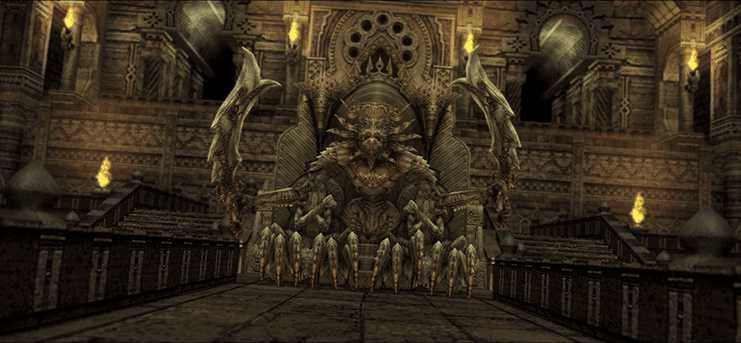
\includegraphics[width=\columnwidth]{./art/tombofraithwall/demonwall2.jpg}
%
\newpage
%
\accf{Parede Demoníaca} é outro guardião da tumba e na luta a seguir, ele se mantém avançando a cada turno, empurrando o grupo ao lado oposto do corredor.
Ele não recebe rodada surpresa, mas age primeiro.
O grupo não pode passar pela Parede Demoníaca, por ela bloquear toda a passagem. Assim, eles tem de lutar ou fugir pela porta do outro lado.
Quando um jogador alcançar a pesada porta dupla, ele tem de usar sua ação e passar um teste de DF~7 para a abrir.
Se falhar, ele só consegue movê-la um pouco, mas o próximo a tentar o mesmo, recebe Vantagem no teste.
Quando a criatura alcançar a porta, ela se fecha e esmaga a todos no caminho.
Após algum tempo, a Parede Demoníaca recua a sua posição original, mas no momento em que o grupo pisa no corredor novamente, ela reaviva e ataca do mesmo modo.
No entanto, ela não recupera PV, então o grupo pode tentar acabar com ela em várias tentativas.
Você pode descrever que partes dela estão desmoronando e quebrando, para se visualizar o dano sofrido.
O grupo não precisa derrotar a criatura de imediato, mas eles terão que fazer isso eventualmente, pois a passagem continuará a ser bloqueada por ela.
A maior vantagem em derrotá-la logo é que o grupo poderá sair, tanto para descansar quanto para comprar mais itens de Dyce.
%
\vfill
%
\ofmonster{Parede Demoníaca}{4}{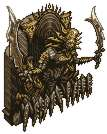
\includegraphics[width=0.2\columnwidth]{./art/tombofraithwall/demonwall.jpg}}
{
	PV: & \hfill 100 & PM: & \hfill 150\\
	FOR: & \hfill 4 & DEF: & \hfill 3 \\
	MAG: & \hfill 3 & RES: & \hfill 4 \\
	AGI: & \hfill 2 & Tamanho: & \hfill G\\
}
{\accf{Espadas}: 2d Danos, \hfill \accf{Deixa:} 1000G, Poção maior\\ \accf{Resistente:}\earth \hfill \accf{Imune:}\poison\sleep\blind \hfill \accf{Fraco:\water}}
{
	\mspell{Envenenar}{6}{0r}{Único}{5u}{O alvo tem que fazer um teste de DF~8 ou ficar Envenenado por 3 rodadas.}{}
	\mspell{Cegar}{6}{0r}{Único}{5u}{o alvo tem que fazer um teste de DF~8 ou ficar Cego por 3 rodadas.}{}
	\mspell{Emudecer}{6}{0r}{Único}{5u}{O alvo tem que fazer um teste de DF~8 ou ficar Mudo por 3 rodadas.}{}
	\mspell{Retardar}{8}{0r}{Único}{5u}{o alvo fica Lento por 3 rodadas.}{}
	\mpassive{Conjuração rápida}{Ao atacar, você pode conjurar um magia em seguida.}
	\mpassive{Empurrar}{Ao se mover adiante, afaste os inimigos em seu caminho. Você pode usar essa habilidade para esmagar os inimigos entre você e a parede ou porta, causando KO de imediato.}
}
%
\clearpage
%
Após passar pela porta, o grupo se encontra em uma câmara chamada de \accf{Câmara real}.
Do outro lado da sala, eles percebem uma porta dupla decorada, a qual ainda não conseguem abrir.
A porta também tem duas cavidades circulares, uma de cada lado.
À esquerda e à direita da sala, há dois lances menores de escadas que levam para baixo.
Além disso, o grupo percebe um mural que foi gravado no chão da sala, mostrando um homem segurando um objeto, um pássaro à sua esquerda e uma parede à sua direita.
A imagem parece representar a criação de Garuda e da Parede demoníaca através do uso do fragmento da aurora.
Ademais, próximo à porta por onde vieram, o grupo percebe um homem ao chão. Ele parece ter sucumbido às suas feridas profundas e olhando melhor, podem deduzir que ele foi vítima da Parede demoníaca.
Da maneira que está vestido, ele dá a impressão de ser um bandido ou ladrão de tumbas, o grupo pode saquear o seguinte dele: uma arma de nível avançado (escolha alguma que um dos jogadores possa usar), 500G e 2 poções.
Para avançar mais, eles devem explorar as passagens da Queda norte e a Queda sul através das escadas nesta sala.
No entanto, antes de partirem, cada jogador recebe mais um \accf{Nível}!
%
\vfill
%
\ofquote{"Mas você deve considerar o prêmio. O fragmento da aurora jaz no interior assim como o tesouro de Raithwall."\\}{Ashe}
%
\vfill
%
\resizebox{\columnwidth}{!}{
	\centering
	\begin{tikzpicture}[]
	\tikzstyle{stairs}=[fill=tombfloor, ultra thick, draw, trapezium, trapezium angle=85, align=center, pattern=horizontal lines]
	\tikzstyle{pillar}=[ultra thick, draw, circle, align=center, fill=tombobstacle, minimum height=0.05\textwidth]
	\tikzstyle{room}=[fill=tombfloor, ultra thick, draw, rectangle, align=center]
	\tikzstyle{door}=[fill=tombobstacle, ultra thick, draw, rectangle, align=center]
	\tikzstyle{sarc}=[fill=tombobject, ultra thick, draw, rectangle, align=center, minimum height=0.05\textheight, minimum width=0.05\textwidth]	
	\tikzstyle{chest}=[fill=tombobject, ultra thick, draw, rectangle, align=center]
	\tikzstyle{statue}=[fill=tombobject, ultra thick, draw, circle, align=center, minimum height=0.03\textheight]	
	\tikzstyle{gargoyle}=[fill=tombobject, ultra thick, draw, circle, align=center, minimum height=0.04\textheight]	
	
	\node[ultra thick, fill=tombwall, draw, rectangle, minimum height=\textheight, minimum width=\textwidth](tarea)at (0,0) {};
	\node[align=center](text)at (0\textwidth, -0.45\textheight) {\bf\LARGE Câmara \bf\LARGE Real};
	
	% northfall	
	\node[align=center](text)at (-0.25\textwidth, 0.475\textheight) {\bf\LARGE Passagem da Queda norte};
	\node[fill=tombfloor, ultra thick, draw, trapezium, trapezium angle=85, align=center, minimum height=0.05\textheight](a1)at (-0.3\textwidth, -0.425\textheight) {};	
	\node[stairs, minimum height=0.05\textheight](a1)at (-0.3\textwidth, -0.425\textheight) {};	
	
	\node[room, minimum height=0.3\textheight, minimum width=0.3\textwidth](a1)at (-0.3\textwidth, -0.25\textheight) {};
	\node[room, pattern=checkerboard, pattern color=gray, draw=none, minimum height=0.25\textheight, minimum width=0.298\textwidth](a1)at (-0.299\textwidth, -0.226\textheight) {};
	\node[room, minimum height=0.3\textheight, minimum width=0.3\textwidth](a1)at (-0.3\textwidth, 0.05\textheight) {};
	\node[room, minimum height=0.25\textheight, minimum width=0.4\textwidth](a1)at (-0.25\textwidth, 0.325\textheight) {};	
	\node[room, minimum height=0.5\textheight, minimum width=0.1\textwidth](a1)at (-0.1\textwidth, -0.05\textheight) {};
	\node[room, minimum height=0.1\textheight, minimum width=0.1\textwidth](a1)at (-0.1\textwidth, -0.35\textheight) {};
	
	\node[door, minimum height=0.01\textheight, minimum width=0.1\textwidth](a1)at (-0.35\textwidth, -0.1\textheight) {};
	\node[door, rotate=90, minimum height=0.01\textheight, minimum width=0.1\textwidth](a1)at (-0.15\textwidth, 0.15\textheight) {};
	\node[door, minimum height=0.01\textheight, minimum width=0.1\textwidth](a1)at (-0.35\textwidth, 0.2\textheight) {};
	
	\node[sarc](a1)at (-0.25\textwidth, -0.025\textheight) {};
	\node[sarc](a1)at (-0.37\textwidth, -0.025\textheight) {};
	\node[sarc](a1)at (-0.25\textwidth, 0.05\textheight) {};
	\node[sarc](a1)at (-0.37\textwidth, 0.05\textheight) {};
	\node[sarc](a1)at (-0.25\textwidth, 0.125\textheight) {};
	\node[sarc](a1)at (-0.37\textwidth, 0.125\textheight) {};
	
	\node[chest, minimum height=0.01\textheight, minimum width=0.1\textwidth](a1)at (-0.1\textwidth, -0.3\textheight) {};
	\node[chest, minimum height=0.025\textwidth, minimum width=0.025\textwidth](a1)at (-0.1\textwidth, -0.35\textheight) {};
	\node[chest, fill=brown, minimum height=0.04\textheight, minimum width=0.025\textwidth](a1)at (-0.075\textwidth, -0.05\textheight) {};
	\node[chest, minimum height=0.04\textheight, minimum width=0.025\textwidth](a1)at (-0.075\textwidth, -0.15\textheight) {};
	
	\node[statue](a1)at (-0.25\textwidth, 0.375\textheight) {};
	\node[chest, minimum height=0.025\textheight, minimum width=0.1\textwidth](a1)at (-0.25\textwidth, 0.325\textheight) {};
	
	%southfall
	\node[fill=tombfloor, ultra thick, draw, trapezium, trapezium angle=85, align=center, minimum height=0.05\textheight](a1)at (0.3\textwidth, -0.425\textheight) {};	
	\node[stairs, minimum height=0.05\textheight](a1)at (0.3\textwidth, -0.425\textheight) {};	
	\node[align=center](text)at (0.25\textwidth, 0.475\textheight) {\bf\LARGE Passagem da Queda sul};
	\node[room, minimum height=0.85\textheight, minimum width=0.4\textwidth](a1)at (0.25\textwidth, 0.025\textheight) {};
	\node[room, minimum height=0.05\textheight, minimum width=0.3\textwidth](a1)at (0.3\textwidth, 0.175\textheight) {};
	\node[door, minimum height=0.01\textheight, minimum width=0.1\textwidth](a1)at (0.1\textwidth, 0.155\textheight) {};
	\node[chest, minimum height=0.01\textheight, minimum width=0.1\textwidth](a1)at (0.35\textwidth, 0.155\textheight) {};
	
	\node[statue](a1)at (0.25\textwidth, 0.375\textheight) {};
	\node[chest, minimum height=0.025\textheight, minimum width=0.1\textwidth](a1)at (0.25\textwidth, 0.325\textheight) {};
	
	\node[gargoyle](a1)at (0.125\textwidth, -0.25\textheight) {};
	\node[gargoyle](a1)at (0.125\textwidth, -0.1\textheight) {};
	\node[gargoyle](a1)at (0.125\textwidth, 0.05\textheight) {};
	\node[gargoyle](a1)at (0.375\textwidth, -0.25\textheight) {};
	\node[gargoyle](a1)at (0.375\textwidth, -0.1\textheight) {};
	\node[gargoyle](a1)at (0.375\textwidth, 0.05\textheight) {};
	\draw[-, color=red!65!black, ultra thick](0.155\textwidth, -0.25\textheight) -- (0.345\textwidth, -0.25\textheight);
	\draw[-, color=red!65!black, ultra thick](0.155\textwidth, -0.1\textheight) -- (0.345\textwidth, -0.1\textheight);
	\draw[-, color=red!65!black, ultra thick](0.155\textwidth, 0.05\textheight) -- (0.345\textwidth, 0.05\textheight);
	
	\node[chest, minimum height=0.04\textheight, minimum width=0.025\textwidth](a1)at (0.2\textwidth, 0.175\textheight) {};
	\end{tikzpicture}
}
%
\newpage
%
\ofquote{"Em vanglória eles se levantaram, bradando desafios aos deuses. Mas, prevaleçer, não conseguiram. A perdição deles foi caminhar na névoa até o fim do tempo."\\}{Fran, recitando uma lenda}\\\\
%
Se o grupo usar as escadas à direita da Câmara real, encontraram a si mesmos dentro de um grande corredor da \accf{Passagem da Queda norte}.
A maioria do piso desta sala tem um padrão quadriculado, com lajotas pretas e brancas, o lado direito da parede é preto, enquanto o esquerdo, branco.
Além disso, a parede esquerda contém uma linha de cavidades em formato de cone de altura aproximada de 1u.
Se investigarem a sala mais detalhadamente, percebem que as lajotas pretas são levemente mais elevadas e as cavidades da parede à esquerda têm buracos em seu centro.
A sala é uma armadilha, assim que alguém pisar em quaisquer lajotas pretas, os cones da parede à esquerda disparam.
Se a armadilha é ativada, cada membro do grupo faz um teste de DF~9 para definir se conseguem evitar os projéteis rápido o suficiente, quem falhar recebe 3d de dano de fogo.
A armadilha pode ser evitada ao se pisar somente as lajotas brancas ou se engatinharem pelo chão.
%
\vfill
%
Depois do corredor, o grupo entra numa câmara maior e vazia, exceto por seis sarcófagos de pedra que estão dispostos pela sala.
Ao entrar, os jogadores veem as palavras \accf{"GUARDIÕES DA ARMADURA"} gravadas no piso.
Uma vez que eles avancem até o outro lado da sala, de repente, os sarcófagos se abrem e um grupo de múmias surgem deles para atacar os personagens.
A quantidade delas deve ser igual ao tamanho do grupo e, na luta a seguir, elas terão uma rodada surpresa.
Entretanto, se os jogadores tentarem investigar os sarcófagos antes, eles terão a vantagem contra as criaturas e serão eles a ter a rodada surpresa.
Depois de as derrotar, eles podem investigar os sarcófagos abertos e encontrarem os seguintes itens: braçadeira poderosa, 2 poções maiores e um super éter.
A sala tem suas saídas, uma à direita e outra oposta à entrada.
%
\vfill
%
\ofmonster{Múmia}{4}{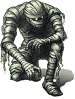
\includegraphics[width=0.18\columnwidth]{./art/tombofraithwall/mummy.jpg}}
{
	PV: & \hfill 38 & PM: & \hfill 0\\
	FOR: & \hfill 2 & DEF: & \hfill 3 \\
	MAG: & \hfill 1 & RES: & \hfill 1 \\
	AGI: & \hfill 2 & Tamanho: & \hfill M\\
}
{
	\accf{Mordida}: 2d Dano \hfill \accf{Deixa:} 300G, poção\\
	\accf{Imune}:\poison\sleep \hfill \accf{Fraco}:\fire 
}
{
	\mspell{Nevasca}{4}{0r}{Único}{3u}{O alvo sofre 2d de dano de Gelo.}{}	
	\mpassive{Toque zumbi}{Sempre que acertar um ataque, o alvo faz um teste de DF 8 ou fica Zumbi por 1~hora.}
	\mpassive{Morto-vivo}{Fique Zumbi permanentemente.}
}
%
\clearpage
%
\ofquote{"Posso ouvir seu chamado..."\\}{Fran}
%
\vfill
%
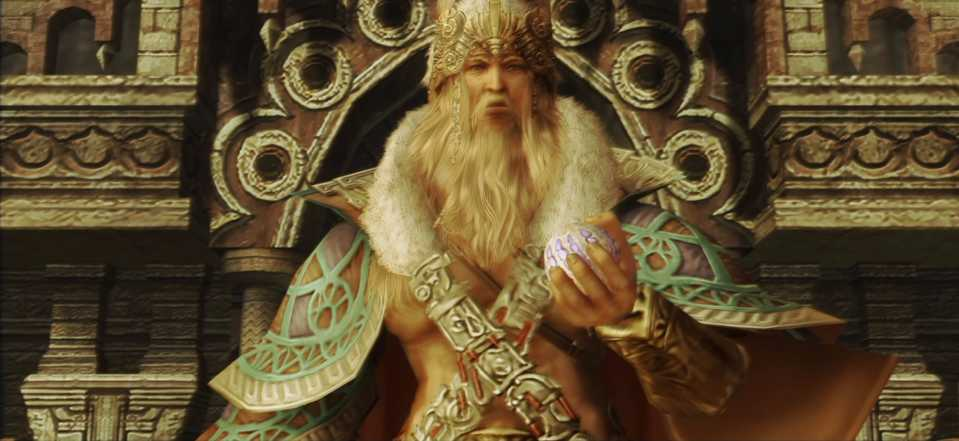
\includegraphics[width=\columnwidth]{./art/tombofraithwall/raithwall.jpg}
%
\vfill
%
Ao passar da porta do lado direito, o grupo entra em um longo corredor e logo percebem dois baús à esquerda.
Um é feito de madeira e sua tranca pode ser facilmente quebrada à força, ele contém uma granada e um éter.
O outro, é feito de metal e não pode ser aberto à força, ao invés disso, os personagens podem tentar arrombar sua tranca ao passar num teste de DF~8.
Depois de o abrir, o grupo encontrar uma matéria de PM+ e uma pena de fênix.
O corredor parece levar a um beco sem saída, mas o final da parede é decorado com imagens impactantes: retratando o rei Raithwall usando uma poderosa magia de fogo contra um monstro.
Ao olhar melhor, percebe-se que o fogo retratado na imagem emite um brilho avermelhado e fraco, provavelmente de origem mágica.
Se causarem algum dano de fogo à parede, um mecanismo mágico é ativado e um pequeno vão se abre na parede, revelando uma sala secreta.
No meio desta sala pequena há um pedestal sobre o qual se encontra um acessório, as abotoaduras de fogo, assim como uma matéria dracônica.
%
\vfill
%
Após caminhar pela porta além dos sarcófagos, o grupo entra numa grande sala com uma estátua em seu centro, com cerca de 2u de altura.
A estátua retrata o rei Raithwall usando armadura pesada e seu braço está esticado como se segurasse uma arma, apesar de vazia.
Em frente a ela há um pedestal com um conjunto de armadura pesada, muito parecida àquela retratada na estátua.
As paredes nesta sala são gravadas com imagens do rei Raithwall lutando contra vários monstros com uma espada longa decorada.
Quando o grupo recupera a \accf{Espada de Raithwall} da passagem da Quedas sul e a põe na mão da estátua nessa sala, eles ouvem um barulho fraco, como se um mecanismo tivesse sido ativado.
Depois de resolver o enigma nesta sala e retornar para a Câmara real, eles percebem que uma das duas gravuras na porta selada agora brilha.
A armadura no pedestal é a \accf{Armadura de Raithwall}, a qual o grupo precisa para a Passagem Quedas sul.
Após resolver o quebra-cabeça completamente e abrir a porta selada, eles podem reivindicar a armadura, que se trata de um equipamento de nível avançado que aumenta o PM máximo do usuário em 10 pontos.
%
\newpage
%
\ofquote{"Chame-me de antiquado, mas eu estava esperando um tesouro cujo valor nós PUDESSEMOS mensurar."}{Balthier}\\\\
%
Se o grupo pegar as escadas à esquerda da Câmara real, eles se encontrarão na \accf{Passagem Queda sul}, que consiste de duas salas.
A primeira é um salão enorme, com duas portas no lado oposto à entrada.
Ao entrar, os jogadores veem as palavras \accf{"GUARDIÕES DA ESPADA"} gravadas no piso.
Em frente ao centro do salão há três pares de estátuas de grandes gárgulas. Além do mais, fracas linhas vermelhas estão desenhadas no chão conectando os pares e, em caso de algum jogador atravessá-las, as duas estátuas de Gárgulas conectadas tomam vida e atacam.
Entretanto, há espaço atrás de cada uma delas, então os jogadores podem passar por trás delas e evitar a armadilha.
Se o grupo alcançar a outra extremidade do salão sem  ativar qualquer estátua, eles escutam um fraco barulho à medida que as linhas vermelhas no chão desaparecem.
Um pequeno compartimento se abre no pedestal das estátuas, que contém o seguinte tesouro: 1.000G, 3 cortinas de luz e 3 cortinas lunares.
%
\ofpar
%
\ofmonster{Gágula}{4}{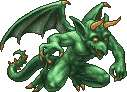
\includegraphics[width=0.27\columnwidth]{./art/tombofraithwall/gargoyle.jpg}}
{
	PV: & \hfill 38 & PM: & \hfill 30\\
	FOR: & \hfill 3 & DEF: & \hfill 2 \\
	MAG: & \hfill 0 & RES: & \hfill 0 \\
	AGI: & \hfill 2 & Tamanho: & \hfill M\\
}
{%
	\accf{Garra}: 2d Dano \hfill \accf{Deixa:} 300G\hfill
	\accf{Resistente}:\earth \hfill \accf{Fraco}:\water
}
{%
	\mspell{Petrificar}{8}{0r}{Único}{5u}{O alvo faz um teste de DF~7 ou fica Imóvel por 3 rodadas.}{}
	\mpassive{Pele de pedra}{Todo dano que sofrer de armas cortantes é reduzido pela metade.}
}	
%
\ofpar
%
Do outro lado do salão, os jogadores se veem em frente à duas portas.
A primeira, à esquerda, é uma porta dupla comum que abre com facilidade, levando a outra sala.
A outra, é feita de pedra maciça e parece diferente de maneira distinta, com várias gravuras decorativas.
Além disso, não parece ter punho ou maçaneta, mas ao invés disso, algo que parece um botão em seu centro.
Se os jogadores investigarem a porta antes de apertar o botão, eles notam que é sua fachada está muito danificada e o piso à direita, em frete a ela há uma quantidade de rachaduras e fraturas incomuns.
Assim que o botão for pressionado. a porta despenca de suas dobradiças de imediato sobre quem estiver em frente a ela.
Todos que forem afetados fazem um teste de DF igual ao seu DF, quem falhar no teste não pode escapar da porta e sofre 4d de dano físico.
Além do mais, todos os alvos que falharem no teste ficam presos sob a porta, mas conseguem se libertar se se esforçarem ou com a ajuda de outros membros do grupo.
A armadilha pode ser evitada ao se encontrar uma maneira de pressionar o botão sem ficar em frente à porta, como arremessar algo nele.
Após a porta ser aberta, o grupo pode entrar numa minúscula câmara detrás, que contém somente um grande baú de madeira sem fechadura.
Ao abri-lo, encontram 500G assim como um acessório Elmo grande. Se os jogadores entrarem no salão noutro momento, eles percebem que a porta parece ter misteriosamente se movido de volta a sua posição original.
%
\ofpar
%
A segunda sala da passagem de Quedas sul, em sua maioria reflete a última sala da passagem Quedas norte, salvo algumas diferenças.
Em primeiro lugar, a estátua do rei Raithwall está no centro desta sala e tem a mesma pose, mas segua uma espada e não veste uma armadura.
Além do mais, uma espada longa jaz no pedestal em frente à estátua.
Por fim, as imagens nas paredes desta sala também representam batalhas do rei Raithwall contra vários adversários, mas o foco está nos méritos de sua armadura, mostrando que suportou a todos os ataques inimigos.
Quando o grupo recupera a \accf{Armadura de Raithwall} da passagem Quedas norte e a põe no corpo da estátua desta sala, eles ouvem um barulho fraco, como se um mecanismo tivesse sido ativado.
A espada no pedestal é a \accf{Espada de Raithwall}, a qual o grupo precisa para a Passagem Quedas norte.
Entretanto, após resolver o enigma por completo e abrir a porta selada, eles podem reivindicar a espada, que é tratada como uma espada de nível Avançado que aumenta o PV máximo de seu portador em 10 pontos.
%
\ofpar
%
Depois de resolver o enigma desta sala e retornar para a Câmara real, eles notam que outra das gravações na porta selada começou a brilhar.
A porta, uma vez trancada, agora leva a Câmara da primeira luz e pode ser aberta.
Ao passar pela porta, todos os membros do grupo têm que realizar um teste de DF~8, quem for bem sucedido tem o pressentimento de que estão sendo observados, mas não sabem o porquê.
%
\vfill
%
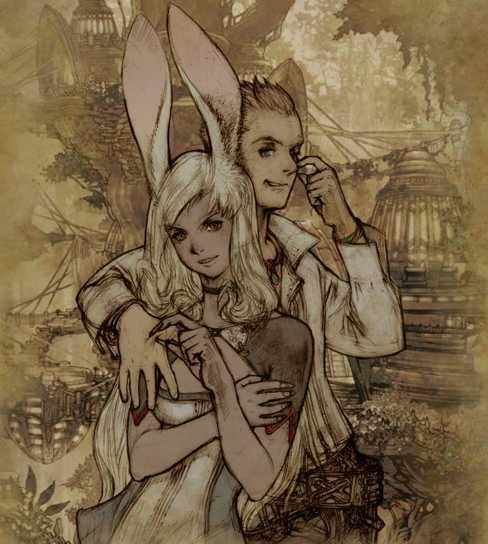
\includegraphics[width=\columnwidth]{./art/tombofraithwall/franandbalthier.jpg}
%
%
\newpage
%
\ofquote{"Minha família conta uma história do rei dinástico e um esper. Dizendo que, em sua juventude, o rei disnástico derrotou um poderoso gigas. Por causa disso, o deus lhe deu ouvidos e, a partir de então, estava ligado ao rei através de servidão."}{Ashe}
%
\vfill
%
\resizebox{\columnwidth}{!}{
	\centering
	\begin{tikzpicture}[]
	\tikzstyle{stairs}=[fill=tombfloor, ultra thick, draw, trapezium, trapezium angle=85, align=center, pattern=horizontal lines]
	\tikzstyle{pillar}=[ultra thick, draw, circle, align=center, fill=tombobstacle, minimum height=0.05\textwidth]
	\tikzstyle{room}=[fill=tombfloor, ultra thick, draw, rectangle, align=center]
	\tikzstyle{stairs2}=[fill=yellow!20!white, ultra thick, draw, rectangle, align=center]
	\tikzstyle{door}=[fill=tombobstacle, ultra thick, draw, rectangle, align=center]
	\tikzstyle{sarc}=[fill=tombobject, ultra thick, draw, rectangle, align=center, minimum height=0.05\textheight, minimum width=0.05\textwidth]	
	\tikzstyle{chest}=[fill=tombobject, ultra thick, draw, rectangle, align=center]
	\tikzstyle{statue}=[fill=tombobject, ultra thick, draw, circle, align=center, minimum height=0.03\textheight]	
	\tikzstyle{gargoyle}=[fill=tombobject, ultra thick, draw, circle, align=center, minimum height=0.035\textheight]	
	
	\node[ultra thick, fill=tombwall, draw, rectangle, minimum height=\textheight, minimum width=\textwidth](tarea)at (0,0) {};
	\node[room, minimum height=0.9\textheight, minimum width=0.9\textwidth](a1)at (0\textwidth, 0\textheight) {};	
	
	%stairs
	\node[stairs2, minimum height=0.225\textheight, minimum width=0.65\textwidth](a1)at (0\textwidth, 0.3375\textheight) {};	
	\node[stairs2, minimum height=0.2\textheight, minimum width=0.60\textwidth](a1)at (0\textwidth, 0.35\textheight) {};	
	\node[stairs2, minimum height=0.175\textheight, minimum width=0.55\textwidth](a1)at (0\textwidth, 0.3625\textheight) {};	
	\node[stairs2, minimum height=0.05\textheight, minimum width=0.5\textwidth](a1)at (0\textwidth, 0.325\textheight) {};	
	
	\node[room, minimum height=0.3\textheight, minimum width=0.4\textwidth](a1)at (-0.25\textwidth, -0.3\textheight) {};	
	\node[room, minimum height=0.3\textheight, minimum width=0.4\textwidth](a1)at (0.25\textwidth, -0.3\textheight) {};	
	\node[room, minimum height=0.1\textheight, minimum width=0.5\textwidth](a1)at (0\textwidth, 0.4\textheight) {};	
	
	\node[door, minimum height=0.01\textheight, minimum width=0.1\textwidth](a1)at (0\textwidth, 0.35\textheight) {};
	\node[door, minimum height=0.01\textheight, minimum width=0.1\textwidth](a1)at (0\textwidth, -0.445\textheight) {};
	\node[door, minimum height=0.01\textheight, minimum width=0.1\textwidth](a1)at (0\textwidth, -0.155\textheight) {};
	\node[door, rotate=90, minimum height=0.01\textheight, minimum width=0.1\textwidth](a1)at (0.05\textwidth, -0.3\textheight) {};
	\node[door, rotate=90, minimum height=0.01\textheight, minimum width=0.1\textwidth](a1)at (-0.05\textwidth, -0.3\textheight) {};
	
	\node[gargoyle](a1)at (0\textwidth, 0.325\textheight) {};
	\node[align=center](text)at (0\textwidth, -0.475\textheight) {\bf\LARGE Câmara Real};
	\node[align=center](text)at (0\textwidth, -0\textheight) {\bf\LARGE Câmara da \\\\ \bf\LARGE Primeira Luz};
	
	\node[pillar](a1)at (-0.25\textwidth, -0.1\textheight) {};
	\node[pillar](a1)at (-0.25\textwidth, 0.05\textheight) {};
	\node[pillar](a1)at (-0.25\textwidth, 0.2\textheight) {};
	\node[pillar](a1)at (0.25\textwidth, -0.1\textheight) {};
	\node[pillar](a1)at (0.25\textwidth, 0.05\textheight) {};
	\node[pillar](a1)at (0.25\textwidth, 0.2\textheight) {};
	
	\node[chest, minimum height=0.025\textheight, minimum width=0.15\textwidth](a1)at (0\textwidth, 0.43\textheight) {};
	\node[chest, minimum height=0.02\textheight, minimum width=0.04\textwidth](a1)at (0\textwidth, 0.4\textheight) {};	
	\node[door, minimum height=0.075\textheight, minimum width=0.04\textwidth](a1)at (0.2\textwidth, 0.4\textheight) {};
	\node[door, minimum height=0.075\textheight, minimum width=0.04\textwidth](a1)at (-0.2\textwidth, 0.4\textheight) {};
	
	%library
	\node[chest, minimum height=0.05\textheight, minimum width=0.04\textwidth](a1)at (-0.4\textwidth, -0.4\textheight) {};
	\node[chest, minimum height=0.05\textheight, minimum width=0.04\textwidth](a1)at (-0.4\textwidth, -0.325\textheight) {};
	\node[door, minimum height=0.075\textheight, minimum width=0.04\textwidth](a1)at (-0.4\textwidth, -0.235\textheight) {};
	\node[door, minimum height=0.02\textheight, minimum width=0.3\textwidth](a1)at (-0.225\textwidth, -0.165\textheight) {};
	\node[door, minimum height=0.02\textheight, minimum width=0.2\textwidth](a1)at (-0.2\textwidth, -0.425\textheight) {};
	
	%armory
	\node[chest, minimum height=0.025\textheight, minimum width=0.1\textwidth](a1)at (0.375\textwidth, -0.175\textheight) {};
	\node[door, minimum height=0.04\textheight, minimum width=0.15\textwidth](a1)at (0.2\textwidth, -0.175\textheight) {};
	\node[pillar, minimum height=0.03\textwidth](a1)at (0.2\textwidth, -0.25\textheight) {};	
	\node[pillar, minimum height=0.03\textwidth](a1)at (0.3\textwidth, -0.25\textheight) {};
	\node[pillar, minimum height=0.03\textwidth](a1)at (0.2\textwidth, -0.35\textheight) {};	
	\node[pillar, minimum height=0.03\textwidth](a1)at (0.3\textwidth, -0.35\textheight) {};	
	\node[door, minimum height=0.015\textheight, minimum width=0.3\textwidth](a1)at (0.25\textwidth, -0.435\textheight) {};	
	\end{tikzpicture}
}
%
\vfill
%
Ao sair da Câmara real, o grupo se vê em um corredor com três portas.
Assim que toma a porta da esquerda, adentram a biblioteca antiga. Embora, todos os livros não tenham suportado ao teste do tempo e estão ilegíveis. Ademais, a sala contém dois baús de madeira, ambos podem ser abertos com facilidade.
Dentro do primeiro está uma Super poção, uma pena de fênix e um super éter. Enquanto no outro, um livro pesado em perfeita condição. Ele conta a história de \accf{Belias o gigas}: Chamado de Gigas por sua aparência: homem e monstro fundidos em um só. Considerado uma falha durante sua criação, recebendo um papel diferente do qual lhe foi pretendido, o Giga desafiou os deuses e perdeu. Desprezado pelos seus antigos mestres, encontrou outro: o rei dinástico, cuja tumba jurou proteger pela eternidade." 
Ao passar pela porta da direita, o grupo entra no que parece ser um arsenal, com suportes de armas e armaduras espalhadas pela sala.
Infelizmente, a maioria dos equipamentos estão inutilizáveis, é possível encontrar algumas peças: um Osso oráculo, uma pele de leão de nemeia e um tridente de níveis avançado.
Sinta-se livre para os trocar por outros equipamentos que sejam mais úteis ao grupo.
%
\clearpage
%
No fim do corredor, o grupo entra em um salão enorme, a \accf{Câmara da primeira luz}.
No lado oposto, uma ampla escadaria leva a um altar no qual os personagens podem ver a estátua de um gigante de quatro braços com chifres de bode, que está sentando com uma lança decorada ao seu lado.
A sala é apoiada por seis pilares decorados, eles podem sentir a imensa quantidade de energia mágica fluindo deles.
Ao se dirigirem à escadaria, a estátua do gigante toma vida, levantando-se aos poucos e sacando sua arma para atacar!
Após ser derrotado, Belias se desintegra em um mar de chamas. O grupo percebe agora que a falta da estátua revela outra câmara pequena, dentro dela está um sarcófago dourado contendo os restos do rei Raithwall.
Vários baús estão espalhados ao redor da sala, contendo ouro e joias, somando 15.000G.
Além disso, há um pedestal decorado em frente ao sarcófago no qual jaz um orb brilhante, o fragmento da aurora. 
O fragmento da aurora é um artefato que pode dobrar o tecido da realidade e pode ser equipado como um acessório, possuindo o seguinte efeito: sempre que você realizar um teste, você pode gastar um Dado de Fortuna 3 ou maior de sua reserva para rolar novamente o teste.
%
\vfill
%
\ofmonster{Belias}{5}{
\includegraphics[width=0.32\columnwidth]{./art/tombofraithwall/belias.jpg}}
{
	PV: & \hfill 90 & PM: & \hfill 150\\
	FOR: & \hfill 4 & DEF: & \hfill 2 \\
	MAG: & \hfill 5 & RES: & \hfill 3 \\
	AGI: & \hfill 2 & Tamanho: & \hfill G\\
}
{	
	\accf{Lança}: 2d Dano, 2u Alcance\hfill \accf{Deixa:} 1.000G\\
	\accf{Resistente}:\earth\fire\dark\holy \hfill \accf{Imune a tudo, Auto-Acelerar}
}
{
	\mspell{Labareda da dor}{20}{1r}{3u}{Você}{Inimigos na área sofrem 4d de dano de Fogo.}{\fire}
	\mspell{Barreira maior}{10}{1r}{Único}{5u}{Ganhe AuDEF e AuRES por 3 rodadas.}{}
}
%
\vfill
%
Subitamente, o grupo ouve a lentos bater de palmas atrás deles e ao se virarem, veem duas pessoas à entrada do salão: \accf{Fran e Balthier}.
Balthier, o homem é um bonito jovem de cabelos castanhos curtos, roupas extravagantes, muito carismático e astuto. Enquanto Fran é um alta e de corpo atlético, tem cabelos brancos e longos, negra e veste uma armadura leve.
Embora seja na maioria humanoide, ela possui características felinas, tais quais longas orelhas e garras.
Ela permanece quieta na maioria do tempo, observando a situação à distância. Ambos são criminosos motivados pela riqueza, mas não são inerentemente maliciosos ou violentos.
Balthier revela que eles entraram na tumba depois do grupo e que os tem seguido desde então. Por fim, pede que lhes entreguem o fragmento da aurora se quiserem sair com vida da tumba.
Nesse ponto, há decisões diferentes que o grupo pode tomar, algumas das quais serão discutidas abaixo.
Mesmo assim, você provavelmente terá de improvisar alguns aspectos dessa sessão final.
%
\newpage
%
\accf{Não entregar coisa alguma:}
Mesmo desejando evitar essa situação, Fran e Balthier sacam suas armas e atacam.
Durante a batalha, eles focam e se manterem afastados com suas armas à distância. Quando necessário, eles se escondem em outras salas para pegar seus inimigos de surpresa. Que acordam horas depois, com os dois sumidos e sem o tesouro e o fragmento da aurora.
Se o grupo ganhar, eles podem decidir o destino dos dois criminosos.
O grupo pode apenas acabar com eles, deixá-los inconscientes ou convencê-los a se juntar a sua causa.
De qualquer maneira, o grupo mantém tanto o tesouro quanto o fragmento da aurora.
%
\ofrow
%
\accf{Entregar o tesouro, mas manter o fragmento da aurora:}
Neste caso, Fran nota que o fragmento perdeu a maior parte de seu poder original e sugere que eles façam um acordo.
Balthier concorda, eles pegam o tesouro e ambos os grupos deixam a tumba e seguem seus caminhos.
%
\ofrow
%
\accf{Convinça-os a juntar forças:}
Para ser bem sucedido, eles têm que fazer os dois acreditarem que uma riqueza ainda maior os espera como membros do grupo.
Se eles conseguirem apresentar uma proposta totalmente convincente, terão que realizar um teste de DF~8 para serem bem sucedidos (o fragmento da aurora pode ser usado).
Se conseguirem, Fran e Balthier se juntam ao grupo e serão controlados pelo MJ. Todos deixam a tuma juntos com o tesouro e o fragmento da aurora.
%
\vfill
%
\ofmonster{Balthier}{5}{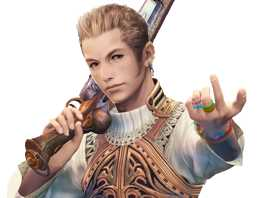
\includegraphics[width=0.3\columnwidth]{./art/tombofraithwall/balthier1.jpg}}
{
	PV: & \hfill 50 & PM: & \hfill 40\\
	FOR: & \hfill 4 & DEF: & \hfill 3 \\
	MAG: & \hfill 0 & RES: & \hfill 1 \\
	AGI: & \hfill 2 & Tamanho: & \hfill M\\
}
{\accf{Arma de fogo}: 2d Dano, 3u Alcance}
{
	\mtech{Mirar: pernas}{8}{0r}{Único}{Arma}{Se acertar um ataque contra o alvo, deixe-o Imóvel por 1 rodada.}{}
}
%
\\\\
%
\ofmonster{Fran}{5}{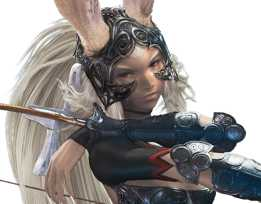
\includegraphics[width=0.28\columnwidth]{./art/tombofraithwall/fran1.jpg}}
{
	PV: & \hfill 45 & PM: & \hfill 45\\
	FOR: & \hfill 3 & DEF: & \hfill 3 \\
	MAG: & \hfill 1 & RES: & \hfill 4 \\
	AGI: & \hfill 3 & Tamanho: & \hfill M\\
}
{\accf{Arco}: 2d Dano, 5u Alcance}
{
	\mtech{Mirar: Braço}{8}{0r}{Único}{Arma}{Se acertar um ataque contra o algo, ele recebe ReFOR e ReMAG por 1 rodada.}{}
}
%
\vfill
%
Após deixar a tumba, o grupo se reune com Dyce à entrada do Vale da morte, ele os encara com espanto ao ouvir das maravilhas que presenciaram dentro da tumba.
Eles ficam no acampamento dele para descansar antes de partir para novas aventuras. Sendo a primeira a deixar a Tumba de Raithwall vivos, o grupo provou que possuem uma força a ser reconhecida e, portanto, recebem um \accf{Nível} a mais!
%
\clearpage